\chapter{\textbf{\textit{Virtual Microfluidics}} enables high-quality single-cell sequencing from a mixed population of cultured bacteria and the human gut microbiome}

This thesis chapter is reproduced from a previously published paper, Xu \textit{et al.}, Nature Methods, 2016.\cite{Xu:2016wt}. Experiments and data analysis on the cultured bacteria were performed by Liyi Xu. Ilana Brito and Liyi Xu conducted the data analysis of the gut microbiome data.

\section{Abstract}
We applied in-gel digital multiple displacement amplification (dMDA) to cultured bacteria and demonstrated whole-genome sequencing of single-cell MDA products with excellent coverage uniformity and markedly reduced chimerism compared with liquid MDA reactions. We demonstrated single-cell sequencing on human gut microbiome samples and obtained 117 pure single draft genomes that enabled the identification of more than 10,000 horizontally transferred genes that have unique population-specific and individual-specific features.

\section{Introduction}
In the burgeoning field of single cell analysis \cite{Blainey:2013hn}, high-throughput and high-fidelity whole-genome \cite{Raghunathan:2005fg,Zhang:2006hq,Fu:2015gl} and whole-transcriptome amplification (WGA and WTA) reactions are needed to produce sufficient material for sequence library construction to support the discovery and validation of new genomes \cite{Marshall:2012jz,Pamp:2012cj,Hess:2011gu}, the analysis of genomic and functional heterogeneity \cite{Wang:2012bb,Fu:2015gl,Pamp:2012cj}.

A variety of approaches have been explored for compartmentalization across a large number of discrete reactors, including SBS plates\cite{Zhang:2006hq}, high-density microfluidic arrays \cite{Love:2013hf}, engineered lab-on-chip systems \cite{Thorsen:2002dn,Landry:2013dh,deBourcy:2014ji,Marcy:2007ip}, and multi-phase micro-droplet systems \cite{Fu:2015gl,Thorsen:2001td,Hindson:2011fg,Morinishi:2015jx}. However, they require complex instrumentation and microfabricated consumables that hinder broad deployment. An ideal platform should resist external contaminants and cross-compartment mixing, exhibit high throughput in small reaction volumes, be stable under temperature change, allow optical access, and allow facile addition and removal of reagents and samples. Finally, it should generate high-quality amplified products and minimize biases and artifacts, such as chimeric fragments commonly formed in PCR, WGA and WTA, that can severely impact single-cell sequencing results. 

Building on my work in Chapter 2 on characterizing \textit{virtual microfluidics} for DNA digital quantification, I further developed the technology for single-cell sequencing. 

\section{Results and Discussion}
\subsection{In-gel single \textit{E. coli} MDA}
We applied digital MDA at the single-cell level using the \textit{virtual microfluidics} system. Individual log-phase \textit{Escherichia coli} could be identified in the hydrogel by fluorescence microscopy (Fig. \ref{fig:EcoliMDA}). We lysed the embedded cells by heat treatment and carried out MDA on the denatured genomic DNA, observing the appearance of MDA clusters at the reaction endpoint 

\begin{figure}
\centering
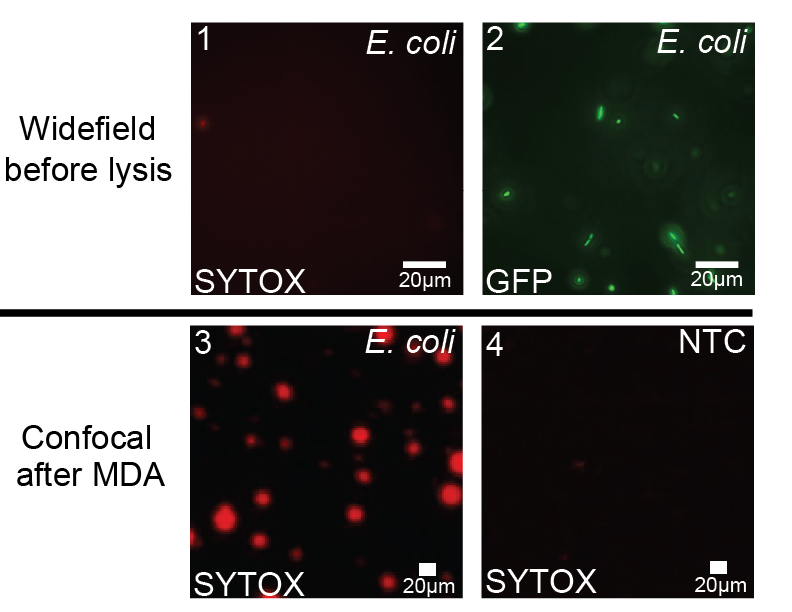
\includegraphics[keepaspectratio,width=0.5\textwidth]{./figures/Thesis-22.png}
\caption[Single-cell MDA on \textit{Escherichia coli}]{Single-cell MDA on \textit{Escherichia coli}. Hydrogel-encapsulated \textit{E. coli}  express GFP and exclude SYTOX Orange before lysis. SYTOX Orange staining reveals product clusters after MDA. Top images are from the same field of view. NTC, MDA control lacking \textit{E. coli} .}
\label{fig:EcoliMDA}
\end{figure}

\subsection{In-gel single-microbe MDA - cultured \textit{E. coli}  and \textit{S. aureus}}
Next, we tested the potential of \textit{virtual microfluidics} to support single-cell shotgun genome sequencing (Fig. \ref{fig:ESMDA}). We mixed log-phase \textit{Escherichia coli} (BL21) and \textit{Staphylococcus aureus subsp. aureus} (RN6390\slash 8325) strains at about 200,000 cells\slash mL and embedded the cells in a 300 micron thick PEG hydrogel. We used a mixed-input approach to ensure sensitive identification of any cross-contamination among single-cell samples and any contamination of single cell samples from other sources (including \textit{E. coli}  DNA contamination). The embedded cells were lysed by enzymatic and heat treatment, and MDA reagents were introduced by diffusion into the gel. 80 sub-samples from the gel (of 60 nL each) were recovered manually in a grid pattern as indicated in Fig. \ref{fig:ESMDA}a Each punch sample was re-amplified to $10^{9}$ - $10^{10}$ overall fold-amplification in a second-round 20 $\mu$L liquid MDA reaction. Real-time PCR (QPCR) assays for \textit{E. coli}  and \textit{S. aureus}  genome sequences were applied to diluted aliquots from each sample (Table \ref{tab:QpcrHydrogel} and \ref{tab:ESprimerList}). The QPCR results were well-approximated by a random cell dispersion model.

% \begin{figure}
% \centering
% 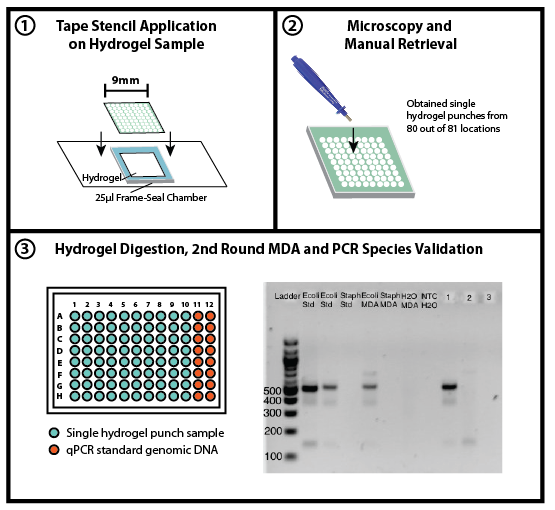
\includegraphics[keepaspectratio,width=0.95\textwidth]{./figures/Figure5A-10}
% \caption[]{.}
% \label{fig:FrameSealPunch}
% \end{figure}

\begin{table}
\centering 
\caption{QPCR characterization of hydrogel punches}
\label{tab:QpcrHydrogel}
\begin{adjustbox}{max width=0.7\textwidth}
\begin{tabular}{c||c} 

\hline 
Total hydrogel punches & 80 \\ 
\hline
\textit{E. coli} positive punches & 7  \\
\hline
\textit{S. aureus} positive punches & 36 \\
\hline
Double positive & 7 \\
\hline
Double negative & 30 \\
\hline
\end{tabular}
\end{adjustbox}
\end{table}


\begin{figure}
\centering
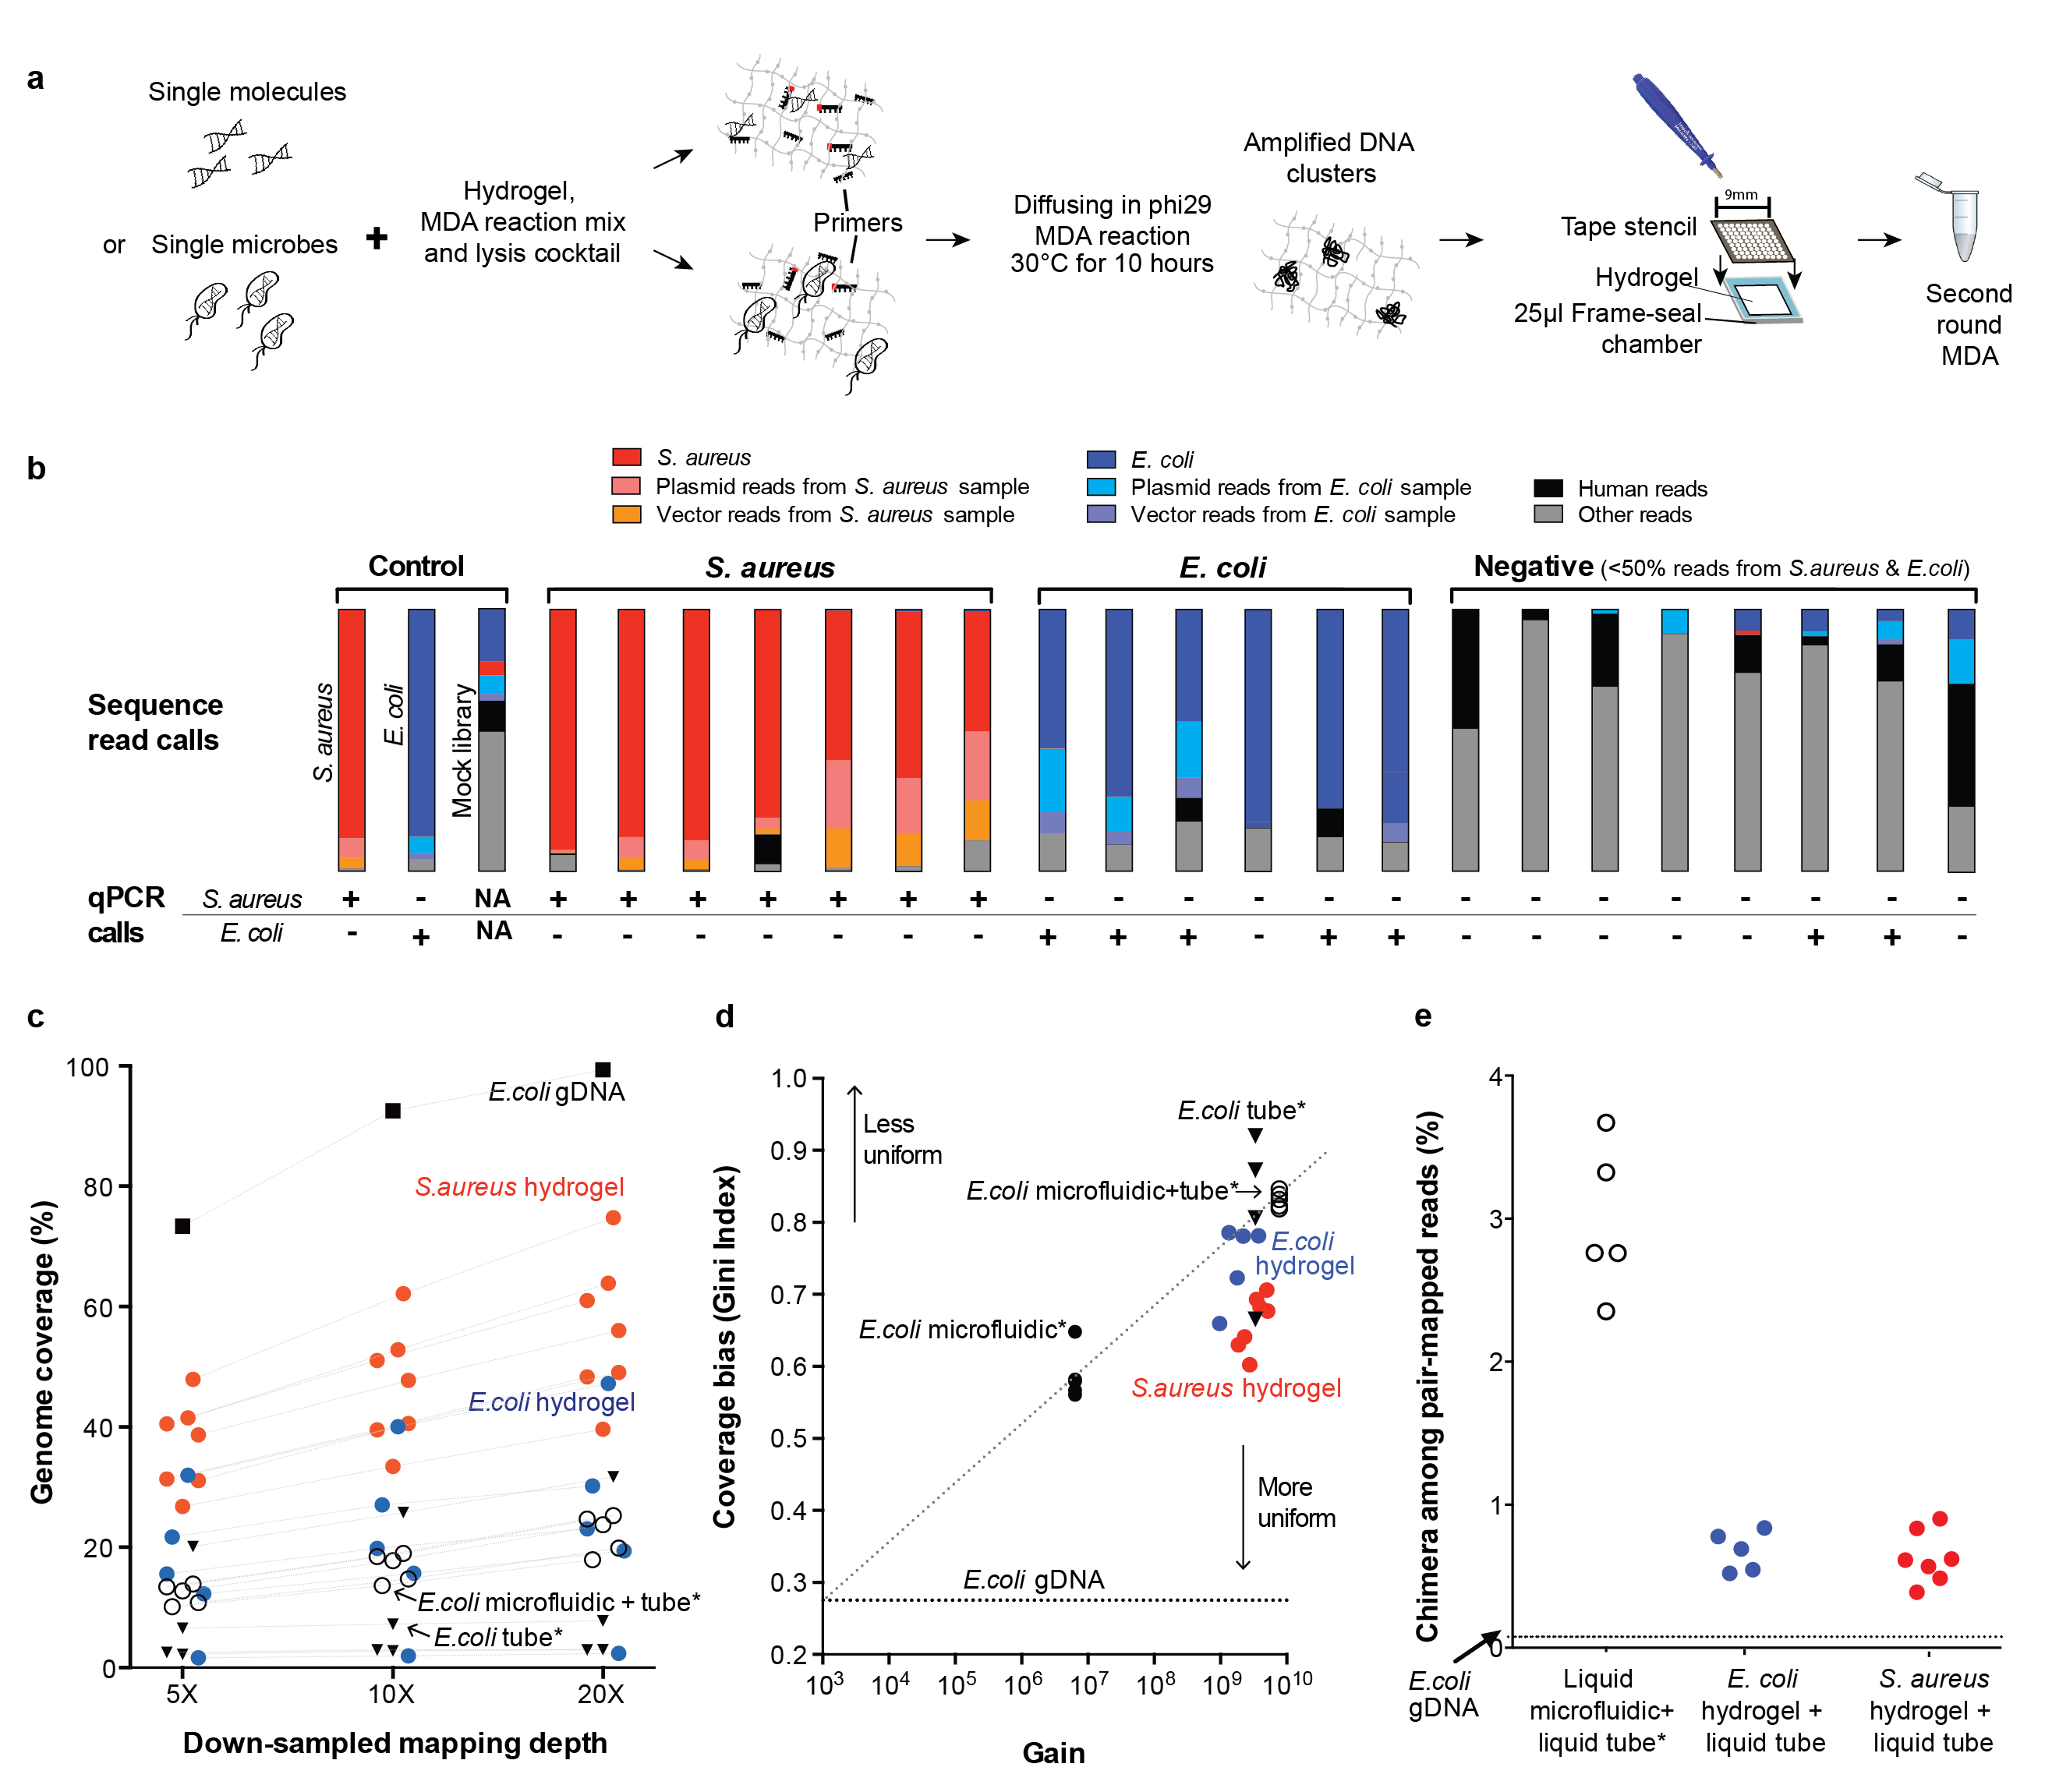
\includegraphics[keepaspectratio,width=0.95\textwidth]{./figures/Thesis-16.png}
\caption[Single-cell whole genome sequencing from \textit{E. coli} and \textit{S. aureus} hydrogel WGA samples.]{Single-cell whole genome sequencing from \textit{E. coli} and \textit{S. aureus} hydrogel WGA samples. (a) \textit{virtual microfluidics} WGA workflow. (b) Sequence read classification using BLAST against the corresponding databases. The samples were ordered based on the ratio of \textit{S. aureus}  to \textit{E. coli}  reads from shotgun sequencing and the fraction of reads not from \textit{S. aureus}  or \textit{E. coli}. Two negative samples are classified as false positive PCR calls. Positive \textit{S. aureus}  and \textit{E. coli}  samples with matching PCR calls are included in downstream analyses. (c) Genome coverage in \textit{S. aureus}  and \textit{E. coli}  hydrogel punch samples compared with published single-cell \textit{E. coli} data produced using conventional liquid MDA reactions*. One \textit{E. coli}  outlier library showed extremely poor genome coverage. This library had low complexity (37 \% duplicate reads), which points to poor library quality rather than MDA as the cause for low genome coverage. (all samples were randomly down-sampled based on mapped reads and bootstrapped 10 times; error in all cases was smaller than the symbols plotted). (d) Coverage distribution bias. Gini Index (derived from Lorenz curve) reports the genome coverage bias of single-cell \textit{E. coli}  and \textit{S. aureus}  punches compared to the same published liquid-MDA single-cell \textit{E. coli}  data as a function of amplification gain. (e) Chimera frequency in the virtual microfluidics samples is significantly reduced versus published \textit{E. coli}  data produced using standard liquid MDA reactions. $\Astericks$ Indicates liquid MDA data from de Bourcy \textit{et al.} 2014.}
\label{fig:ESMDA}
\end{figure}

We sequenced Illumina short-insert libraries produced from randomly selected punch samples and positive-control gDNA samples (MiSeq v2 500 cycles). Quality-filtered reads were then mapped to \textit{de novo} assemblies of the positive-control gDNA datasets and sequence databases (Table \ref{tab:MapStatES}, Table \ref{tab:deNovoAssemblyES}). The positive punch samples showed strong enrichment (Fig. \ref{fig:ESMDA}b) for reads mapping to the expected reference genome (Fig. \ref{fig:MappingES}) while the negative punch samples showed enrichment for human reads, reads with poor mapping quality, and \textit{E. coli} (possibly contaminants from the reagents and\slash or laboratory environment), and were similar to the results from a mock library (Table \ref{tab:OtherReadsES}). The lack of \textit{E. coli}  and \textit{S. aureus} cross-contamination in the positive punch samples indicates that \textit{virtual microfluidics} can resolve single-cell amplification products.

At 20$\times$ mean coverage (Table \ref{tab:DownsamplingESD}), approximately 30 \% of the \textit{E. coli}  genome and about 60 \% of the \textit{S. aureus}  genome were covered in each single-cell sample (Fig. \ref{fig:ESMDA}c). The coverage values for \textit{E. coli}  are in-line with typical single microbe genome sequencing at similar sequencing effort \cite{Woyke:2011eg,deBourcy:2014ji}. The superior coverage performance in \textit{S. aureus}  may be attributable to the lower GC content of \textit{S. aureus}  (33 \%) compared with \textit{E. coli}  (51 \%), better accessibility (deproteination) of the genome after lysis, and\slash or higher average genome equivalents per cell in \textit{S. aureus} resulting from cell cycle dynamics.

To rigorously evaluate sequence coverage distribution, we calculated the Gini Index (a measure of inequity ranging from 0 to 1) for each of our single-cell datasets and previously published single-cell \textit{E. coli} liquid MDA datasets for which raw read data were available and fold-amplification was known(Fig. \ref{fig:ESMDA}d). The coverage uniformity in our single-cell punch samples compares favorably with published single-cell datasets at similar amplification gain.

We then analyzed the occurrence of chimeric reads, which are known to occur with high frequency in MDA by a cross-priming mechanism \cite{Lasken:2007db}. Chimeric reads directly confound \textit{de novo} assembly, analysis of rearrangements, and mapped read counting. Our single-cell datasets contained about 0.5 \% chimeric reads, approximately five-fold lower than previously published short-read datasets produced using liquid single-cell MDA samples (Fig. \ref{fig:ESMDA}e and Table \ref{tab:MapStatES}). The occurrence of chimeric reads spanning more than 10 kb of the template is even lower (about 0.1 \%, Fig. \ref{fig:Chimera10k}), raising the possibility of extracting long-range information from single-cell MDA samples using long-read sequencing. This dramatic reduction in the occurrence of chimeric reads can be understood by restricted diffusion of the MDA intermediates that prevents cross-priming by isolating each portion of the product mixture. It may be the case that substantially all of the chimeras we observed in the punch samples were generated during the liquid-phase secondary amplification reactions. Based on these results, it is likely beneficial to run MDA in PEG hydrogels for all applications at all scales. 

\begin{figure}
\centering

\includegraphics[keepaspectratio,width=\textwidth]{./figures/SuppFig8.jpg}
\caption[MDA chimera frequency with different insert sizes, \textit{E. coli} and \textit{S. aureus} data]{MDA chimera frequency with different insert sizes, \textit{E. coli} and \textit{S. aureus} data. a) 1 - 3 kb. b) 3 kb - 10 kb. c) Larger than 10 kb. Centerlines represent the mean value.}
\label{fig:Chimera10k}
\end{figure}

\subsection{In-gel single-microbe MDA - human gut microbiome samples}
Next, we tested the potential of \textit{virtual microfluidics} for single-cell genome sequencing using samples from the Fiji Community Microbiome project (FijiCOMP). The FijiCOMP samples contain a vast uncharacterized diversity of microbial species that differ from those found in the microbiome of Western subjects. The procedure for processing these human stool samples was similar to those for lab-cultured \textit{E. coli} and \textit{S. aureus}, with modifications for initial sample processing and lysis (methods).

\begin{figure}
\centering
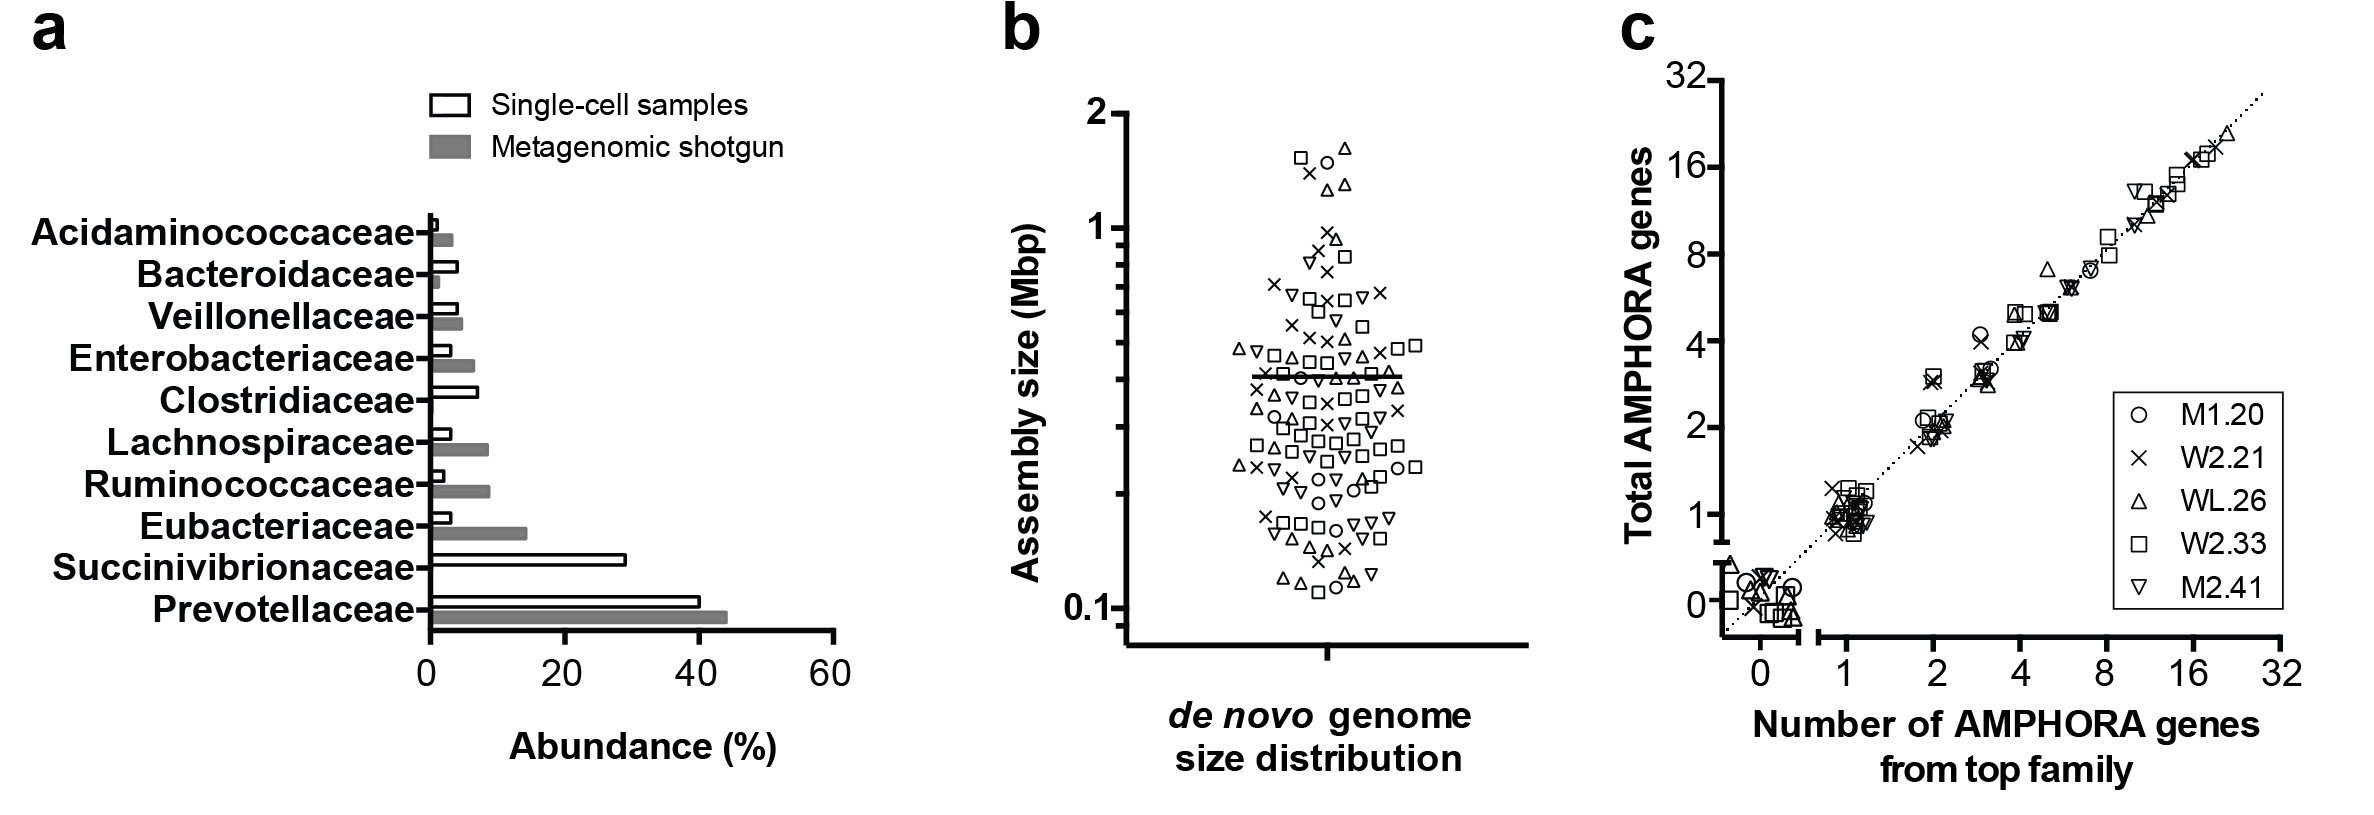
\includegraphics[keepaspectratio,width=1\textwidth]{./figures/Thesis-23.png}
\caption[Fiji microbiome project (FijiCOMP) single-cell whole-genome sequencing.]{Fiji microbiome project (FijiCOMP) single-cell whole-genome sequencing. Here are the results for 117 single-cell data sets from five donor individuals. (a) Distribution of top ten microbial families from single-cell assemblies and metagenome shotgun sequencing. Samples were weighted according to the number of single cells analyzed (Table \ref{tab:MetagenomicFiji}). (b) \textit{De novo} assemblies from single-cell sequencing data ranged from 100 kbp to 2 Mbp. The line indicates the mean assembly size. (c) The total number of AMPHORA genes is nearly equal (dotted line) to the number of AMPHORA genes from the top phylogenetic family for each sample, supporting the assertion that each data set arises from an individual bacterial cell. A Gaussian-distributed random jitter ($\mu$ = 0, $\sigma^{2}$ = 0.1) was applied to enhance visualization.}
\label{fig:Amphora}
\end{figure}

\begin{table}[h]
\centering 
\caption{Overview of 117 FijiCOMP single-cell hydrogel samples}
\label{tab:Fiji117cells}
\begin{adjustbox}{max width=\textwidth}
\begin{tabular}{c|c}
\hline 
Sample categorizations & Number of punches \\
\hline\hline
Low read counts; no assembly & 16 \\
Laboratory contamination (\textit{E. coli}, \textit{P. aeruginosa}) & 29 \\
Human cell sequences amplified & 3 \\
No phylogenetic markers & 80 \\
Enrichment of multiple taxonomies from assemblies & 108 \\
Assembly < 100kb & 68 \\
\hline
\cellcolor{lightgray}Single-cell assemblies & \cellcolor{lightgray}117 \\
\hline
Total sequenced & 421 \\ \hline
\end{tabular}
\end{adjustbox}
\end{table}

We processed a total of 421 hydrogel punch samples and compared the distribution of organisms detected in our hydrogel samples with the distribution observed from shotgun metagenomic profiling, which showed that the same top microbial families were observed using both approaches (Fig. \ref{fig:Amphora}a and Table \ref{tab:MetagenomicFiji}). Interestingly, the second most abundant microbial family found in the single-cell dataset, the Succinivibrionaceae, was not initially detected (but later confirmed) in the shotgun metagenomic data due to its rare representation in the established database (using standard methods for the taxonomic assignment such as MetaPhlAn \cite{Segata:2012ts}). This discrepancy highlights the importance of unbiased approaches like single-cell analysis for organisms that are less well represented in reference databases.

We carried out de novo assembly of the single-cell datasets and assigned taxonomy to ribosomal gene sequences and 31 \say{single copy} bacterial marker genes (at the family level) \cite{Wu:2012dh}. This analysis enabled us to make crude assessments of genome coverage and sample purity in the FijiCOMP single-cell datasets (for which we lack strain-specific bona fide reference sequence). Of the 293 assemblies (up to 12 Mbp), we classified 117 as single amplified genomes with assembly size greater than 100 kb and strong enrichment of sequences from a single taxonomy (Fig. \ref{fig:Amphora} and see Table \ref{tab:Fiji117cells}) for the fate of all samples. The purity of single amplified genomes are evaluated with the identity of AMPHORA (AutoMated PhylogenOmic infeRence Analysis) marker genes. AMPHORA genes are a collection of protein-coding marker genes that are single-copy in the genome, universally distributed, and are relatively recalcitrant to horizontal gene transfers \cite{Wu:2012dh}. We identify the number of AMPHORA marker genes and their phylogenines in each single amplified genome. If the total number of AMPHORA genes is nearly equal to the number of AMPHORA genes from the top phylogenetic family, it indicates the dataset arises from an individual bacterial cell (Fig. \ref{fig:Amphora} c). Overall, the data quality observed from these human microbiome bacteria was consistent with the results of our studies with lab-cultured Gram-negative and Gram-positive samples and demonstrates the applicability of the hydrogel method to real-world samples, including lysis and amplification of a variety of naturally occurring microbes.

% In order to test our hypothesis that mobile genes are distributed without geography barrier and interpersonal and intraperson distance. We conducted mobile gene transfer analysis on 117 single-cell datasets. The species information is obtained from with RNAMMER on available 16S or 5S sequence. For cells that lack a 16S sequence, the species is defined by AMPHORA call and the 16S sequence was obtained through RDP. All available 16S sequences was concatenated and the phylogeny distance matrix between all pairs of 16S sequences were calculated using USEARCH \cite{Edgar:2010cv}. The goal was to find distantly related genomes (less than 97\% 16S rRNA similarity). HGT is the best explanation for these because the highly conserved 16S gene evolves about 25-fold more slowly than protein-coding synonymous sites \cite{Smillie:2011jc,Ochman:1999to}. Vertically inherited orthologues should be nearly saturated with wobble basepair mutations in such divergent genomes. After identifying the single cells that are more than 3\% distant, we identified protein-encoding genes for each selected single cells using RAST \cite{Aziz:2008ku}. Each cell's genes were pairwise matched using USEARCH to look for genes that are 100\% identical. We categorize these genes as horizontally transferred genes (HTG). Next, the HTG set is mapped to the database to identify antibiotic resistant genes, virulence factors(VF), insertion sequences and phages. We expect the percent of HGT pairs (pairs of genomes that have more than one 100\% identical genes) to decrease as 16S distance increases from 3\% to 30\%. We also want to find out the difference in numbers and distributions of antibiotic resistant and VF HGTs between different persons and within the same person. In addition, among the shared genes across all Prevotellaces family, we made a phylogeny tree to show the divergence of genes.

\subsection{Random Dispersion Model}
The expected number of punches that have both \textit{E. coli}  and \textit{S. aureus}  is (based on qPCR analysis of the 80 punches): 

\begin{aligned}
	&P_{\textit{E.coli}} = \frac{14}{80} = 0.175 \\
	&P_{\textit{S.aureus}} = \frac{43}{80} = 0.538 \\
	&P_{negative} = \frac{30}{80} = 0.375 \\
	&< N_{both \textit{E.coli} and \textit{S.aureus}} > = \frac{14}
{80} \times \frac{43}{80} \times 80 = 7.52\\
\end{aligned}


This result is in line with our qPCR result of seven double positive punches (Table \ref{tab:QpcrHydrogel}), indicating the likelihood that the distributions of \textit{E. coli}  and \textit{S. aureus}  across the punch samples are independent as we expected. Furthermore, if we assume a random (Poisson) distribution of microbes in the hydrogel: 

\begin{aligned}
	&P_{\textit{E.coli}}\ (0, \lambda_E) = e^{- \lambda_E} = \frac{66}{80} = 0.825 , \ \lambda_E = 0.192 \\
	&P_{\textit{E.coli}}\ (1, \lambda_E) = \lambda_E \ e^{- \lambda_E} = 0.158 \\
	&P_{\textit{E.coli}}\ (2, \lambda_E) = \frac{\lambda_E^2 \ e^{- \lambda_E}}{2} = 0.01 \\
	&P_{\textit{E.coli}}\ (Single\ cell) = \frac{0.158}{1-0.825} = 90.3\% \\
	&P_{\textit{S.aureus}}\ (0, \lambda_S) = e^{- \lambda_S} = \frac{37}{80} = 0.462 , \ \lambda_S = 0.772 \\
	&P_{\textit{S.aureus}}\ (1, \lambda_S) = \lambda_S \ e^{- \lambda_S} = 0.356 \\
	&P_{\textit{S.aureus}}\ (2, \lambda_S) = \frac{\lambda_S^2 \ e^{- \lambda_S}}{2} = 0.138 \\
	&P_{\textit{S.aureus}}\ (Single\ cell) = \frac{0.356}{1-0.462} = 66.2\% \\
\end{aligned}


The low probability value for the occurrence of single \textit{S. aureus} is calculated based on the high number of hydrogel punches that were identified as \textit{S. aureus} by qPCR. To bring down the value, a more dilute sample of \textit{S. aureus} should be used (Table \ref{tab:RandomDispersion}). 

\begin{table}[h]
\centering 
\caption{Microbe occurrence probability}
\label{tab:RandomDispersion}
\begin{adjustbox}{max width=0.8\textwidth}
\begin{tabular}{c||ccc}
\hline 
 & P_{\textit{E.coli}}(0)=0.825 & P_{\textit{E.coli}}(1)=0.158 & P_{\textit{E.coli}}(2)=0.01 \\
\hline\hline
P_{\textit{S.aureus}}(0)=0.463 & 0.38 & 0.073 & 0.0046 \\
P_{\textit{S.aureus}}(1)=0.356 & 0.29 & 0.056 & 0.0036 \\
P_{\textit{S.aureus}}(2)=0.138 & 0.114 & 0.022 & 0.0014 \\
\hline
\end{tabular}
\end{adjustbox}
\end{table}

\section{Conclusion}
\textit{Virtual microfluidics} enables high throughput whole genome amplification and serial reagent exchange in an easy-to-use, benchtop format that requires no special equipment or environmental control. Here we show preparative amplification and recovery of single bacterial genomes for \textit{ex-situ} analysis of lab-cultured control cells and the human gut microbiome by next-generation sequencing (NGS).

\textit{Virtual microfluidics} establishes a new paradigm in single-molecule and single-cell analysis with dramatically different characteristics than established microfluidic approaches. Besides reducing the production of chimeras in MDA, the unique physical characteristics of the engineered hydrogel environment may provide a means for enhancing coverage extent and uniformity from WGA and WTA samples through the self-limiting reactivity within each virtual compartment, similar to a recently reported emulsion approach \cite{Fu:2015gl}. In addition, the straightforward addition and removal of reagents to/from product clusters \textit{en masse} and excellent optical access ideally suit the \textit{virtual microfluidics} system for rare-cell assays incorporating \textit{in situ} labeling of cells or product clusters. We expect that \textit{virtual microfluidics} will find application as a high-throughput platform for single-cell sample preparation.

% Talk about environmental microbiome field work 

\section{Materials and Methods}
\subsection{In-gel single-microbe MDA - cultured \textit{E. coli}  and \textit{S. aureus} }
Antibiotic resistant \textit{Staphylococcus aureus subsp. aureus} (GFP) NCTC 8325 and \textit{Escherichia coli} (RFP) BL21 strains were obtained as cryogenic stocks. For each culture, the frozen stock was inoculated in 5 mL LB broth and cultured at 37 $^{\circ}$C overnight. 10 $\mu$L of 25 mg\slash mL Chloramphenicol was added to \textit{S. aureus}  culture and 5 $\mu$L of 50 mg\slash mL Ampicillin was added to the \textit{E. coli}  culture. 50 $\mu$L and 20 $\mu$L of each overnight culture were added to fresh 5 mL LB broth with the respective antibiotic concentration. After two hours incubation (to achieve exponential growth phase), 1 mL of each culture (O.D. 600 nm = 0.2) were centrifuged for 2 min at $>$10 krpm and the pellet was washed with 500 $\mu$L PBST (1\% Tween--20) twice. The equal ratio mixture of microbes were diluted to 206,000 cells\slash mL and 1 $\mu$L of each was encapsulated in the same hydrogel sample to produce an average of less than 1 microbe per 500 $\mu$m diameter view. In addition to hydrogel MDA reaction mix described above, lysozyme (Sigma, final concentration 2.5 mg\slash mL) and lysostaphin (Sigma, final concentration 0.1 mg\slash mL) were added to the mix. The hydrogel was left at RT to let crosslink for 20 mins and cross-linked hydrogels were incubated at 37 $^{\circ}$C for 1 hour for microbe lysis and heated to 95 $^{\circ}$C for 5 min to denature genomic DNA before rapid quenching on ice. 1 $\mu$L of REPLI-g sc Polymerase (Qiagen) diluted in 2 $\mu$L water was then added on top of the hydrogel and allowed to diffuse into the gel. Next, the gel chamber is resealed and MDA was conducted for 10 hours. After the MDA reaction, the sample was heated to 65 $^{\circ}$C for 5 min to deactivate phi29 polymerase.

\subsection{Image acquisition and analysis}
Z stack images were taken by Nikon ultra-fast laser scanning confocal microscope with pinhole = 1.2, HV = 112, offset = 0, laser wavelength = 561 nm, laser power = 1.3 to 1.5, using a 20$\times$ objective on Galvano mode. Acquisition speed was 1 frame\slash sec and z step size was 0.95 $\mu$m. On the inverted microscope, z stack images were taken with the exposure time 100 ms, Lumencor excitation power 10 \%, binning size 2 and z step size 10 $\mu$m. Both z Stacks were first processed into max intensity projections in FIJI(FIJI is just image J). Max projection tif files were then loaded into MATLAB. Background was obtained by applying a Gaussian filter of hsize 200 and sigma 50. All max projections were background-subtracted and thresholded at 2$\times$ \textendash 2.5$\times$ standard deviations above the mean intensity. Cluster count, cluster area (radius), and cluster mean intensity were obtained with the bwconncomp and regionprops functions.

For whole gel (25 $\mu$L, 9mm by 9mm) microbe density approximation, I imaged the gel with a 4$\times$ objective in a 5 $\times$ 5 grid with a 31 \% overlap. The 25 images were stitched using the FIJI stitching function. Fluorescent DNA clusters were counted and only gels with the appropriate clusters' range and dispersion (60 $\sim$ 80 per gel) were selected for hydrogel cluster retrieval. Images of the sampled locations were acquired but not used to guide sampling, sample preparation, or data analysis in this case.

\subsection{MDA product cluster retrieval}
In order to identify and retrieve a regular array of punches (not guided by cluster image data), we produced a tape stencil to guide the punch tool (Adhesive Applications High Tack Silicone Film Tape). We laser cut the double-sided tape with a 9 $\times$  9 array of 500 $\mu$m diameter circles that has a center-to-center distance of 947 $\mu$m (Full Spectrum Laser LLC MLE--40). The tape stencil was applied on top of the frame seal plastic cover. The gel was peeled off the glass slide by allowing it to adhere to the plastic cover. The gel is then punched with a 1 mm diameter steel punch (Militek) and the micro-samples collected in a 96 well lobind twinteck plate (Eppendorf). The steel punch was cleaned with bleach and 70 \% Ethanol after each use.

\subsection{BLAST analysis and read assignment for \textit{E. coli} and \textit{S. aureus}}

\begin{figure}
\centering
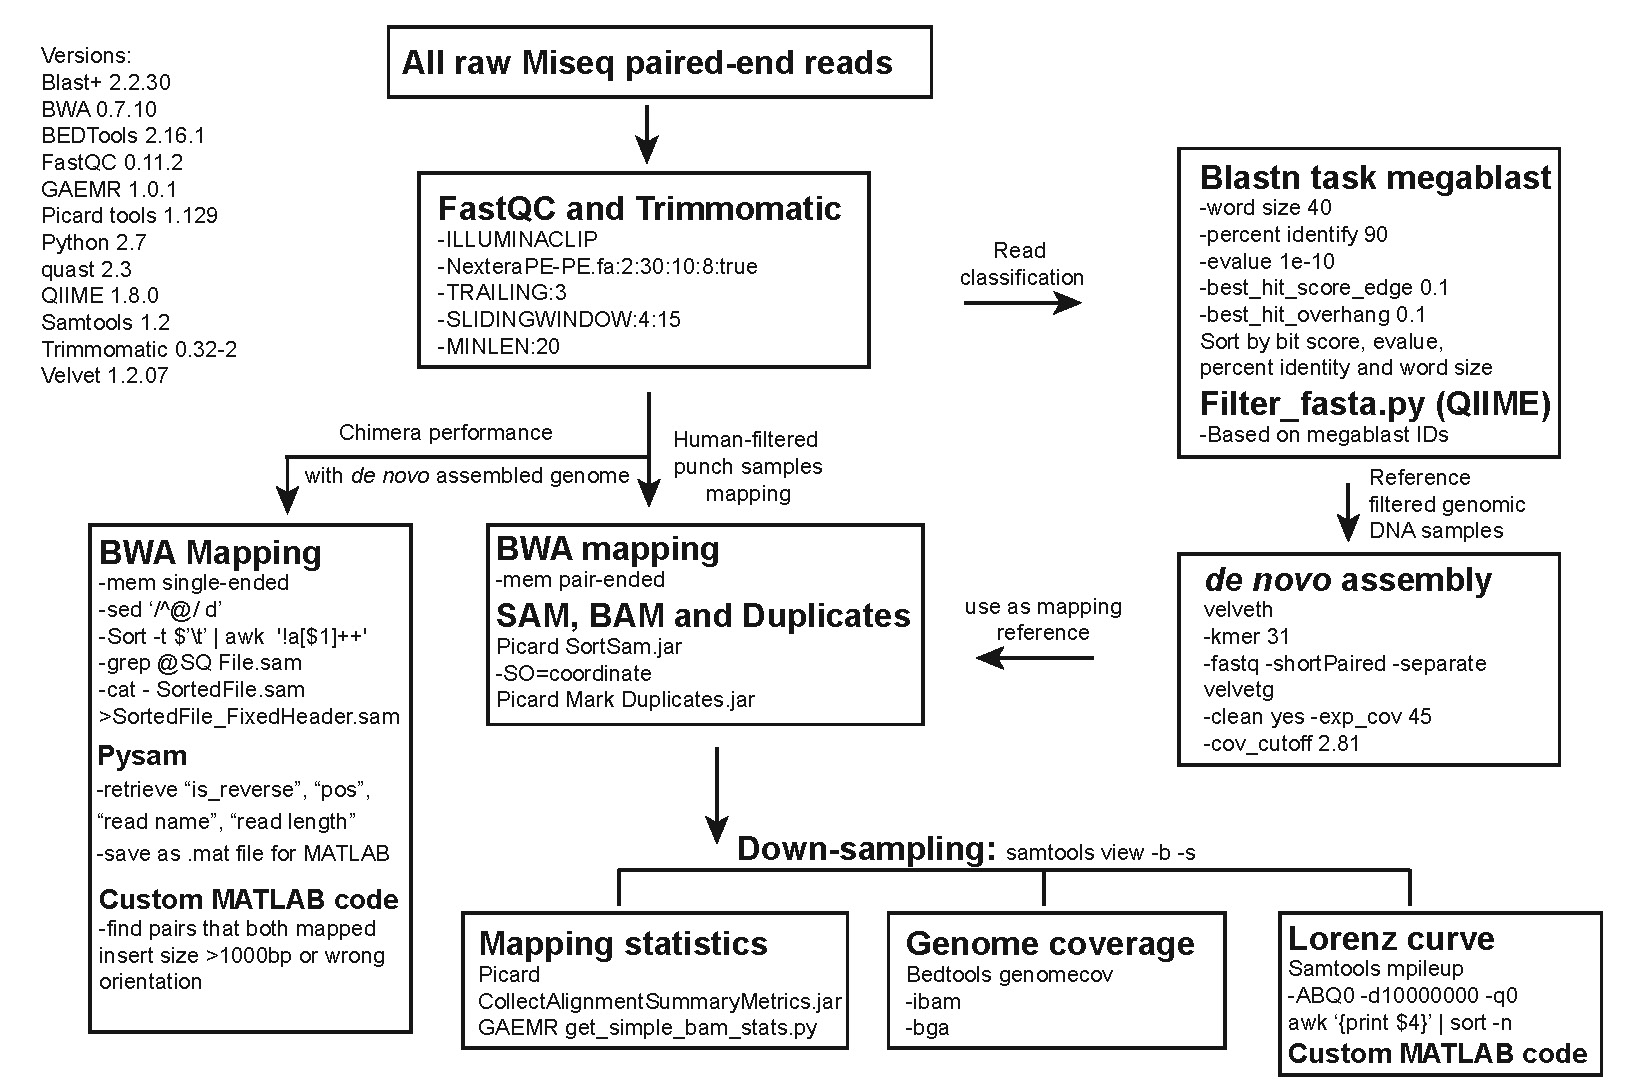
\includegraphics[keepaspectratio,width=1\textwidth]{./figures/SuppFig6.jpg}
\caption[NGS data analysis schematic for \textit{E. coli} and \textit{S. aureus}]{NGS data analysis schematic for \textit{E. coli} and \textit{S. aureus}. The analysis workflow is shown with a combination of bioinformatic tools, python scripts and MATLAB scripts.}
\label{fig:ESDataAnalysis}
\end{figure}

To characterize all samples after quality trimming, each sample (R1 from each read pair) was blasted (task megablast) with the parameters listed in Fig. \ref{fig:ESDataAnalysis}. The BLAST database for \textit{E. coli} consists of three \textit{E. coli} genomes (strain BL21, MG1655 and W3110). The \textit{S. aureus} database consists of the genomes of strain 8325, TW20 and USA300. Univec, Plasmid and Human genome (GRCH38) databases were downloaded from NCBI. All databases were produced using makeblastdb and blastdb\_aliastool. Each read was mapped to all five databases (\textit{E. coli}, \textit{S. aureus}, Univec, Plasmid, and Human db) and the results were ranked based on bit score, e-value and then percent identity. We assigned each read to one of the source databases based on the top hit. Using the filter\_fasta.py tool in QIIME  \cite{Caporaso:2010jf}, we selected reads that did not map to any of the five databases for further analysis. We ran BLAST against the nt database to characterize these reads (Table. \ref{tab:OtherReadsES}). 

\begin{table}
\caption{Sequence read classification \say{other reads}, \textit{E. coli} and \textit{S. aureus}}
\label{tab:OtherReadsES}
\begin{center}

\includegraphics[width=\linewidth]{./figures/OtherReadsClassificationES}
\end{center}
\end{table}

\subsection{Secondary liquid MDA and PCR screening - cultured \textit{E. coli} and \textit{S. aureus}}
The retrieved hydrogel punch (approximately 0.06 $\mu$L of hydrogel and 10 pg of DNA if a cluster was captured) was dissolved and denatured in 1 $\mu$L of 1 M KOH with 0.1 mM EDTA and 0.1 M DTT at 72 $^{\circ}$C for 10 min before neutralization in 1 $\mu$L stop solution (Qiagen REPLI-g single cell kit). The neutralized product was added to 12.5 $\mu$L REPLI-g sc reaction mix with 1 $\mu$L of phi29 polymerase. The secondary MDA reaction was incubated for 10 hours before polymerase deactivation at 65 $^{\circ}$C for 5 min. The DNA products from MDA were cleaned by the SPRI procedure in 1.8:1 beads to DNA volume (Beckman Coulter). Each sample was analyzed for the presence of \textit{S. aureus} and \textit{E. coli} marker loci by four sets of primers (Table \ref{tab:ESprimerList}) in standard qPCR reactions with Jumpstart Taq 2$\times$ ready mix (Sigma Aldrich), 1$\times$ Evagreen (Biotium), 1$\times$ ROX (Invitrogen) and 1 $\mu$M primers in Stratagene M3005. Both melting curve analysis and agarose gel electrophoresis (not shown) were used to support the QPCR results.

\begin{table}
\caption{PCR primer sequences}
\label{tab:ESprimerList}
\begin{center}
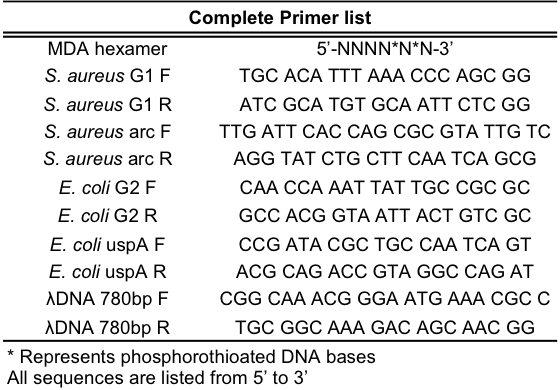
\includegraphics[width=0.5\linewidth]{./figures/ESprimerList}
\end{center}
\end{table}

\subsection{WGS library construction \& sequencing}
We quantified the purified MDA products using the Qubit\slash Quant-IT HS assay (Thermo Fisher Scientific) and normalized samples to 5 ng\slash $\mu$L. All SPRI procedures were conducted on the Bravo robotic system (Agilent Technologies). 5 ng of purified DNA was then added to 1 $\mu$L of 5$\times$ tagmentation DNA buffer, 2 $\mu$L H2O and 1 $\mu$L Nextera Tagmentation DNA enzyme (Illumina). The mixture was first incubated at 58 $^{\circ}$C for 10 min. With the addition of 0.5 $\mu$L of 1 \% SDS, it was then incubated at 68 $^{\circ}$C for 10 min, 4 $^{\circ}$C for 3 min and 25 $^{\circ}$C for 3 min to stop the tagmentation reaction. Another SPRI clean-up was carried out, followed by PCR library barcoding using Index primer N7 and S5 (Illumina) with the thermal protocol: 72 $^{\circ}$C for 3 min, 98 $^{\circ}$C for 30 sec, 12 cycles of 98 $^{\circ}$C for 10 sec, 60 $^{\circ}$C for 30 sec, 72 $^{\circ}$C for 30 sec and a 5 min final extension at 72 $^{\circ}$C. Samples were barcoded uniquely in the PCR step using standardized custom sample barcodes (Broad Institute Genomics platform). The PCR products were purified with SPRI twice with 1:1 beads to DNA volume and library quantification was carried out with the Quant-It assay (Thermo Fisher Scientific) and the KAPA library quantification kit (KAPA Biosystems). Library normalization and pooling were conducted on the Janus Mini Varispan workstation (PerkinElmer). For \textit{E. coli} and \textit{S. aureus} samples, an average of 0.7 million paired-end reads were allocated for each sample in a MiSeq 500 cycle v2 run (Illumina). For stool samples, about 1 M reads ($>$ 50$\times$) were allocated to each sample on HiSeq 2500 2$\times$ 101\slash 125 runs (Illumina). 

\subsection{NGS data analysis for \textit{E. coli} and \textit{S. aureus}}
Data quality was first visualized using FastQC (Babraham Bioinformatics). All data were trimmed using trimmomatic \cite{Bolger:2014ek} and human reads were filtered out with BLAST and QIIME. Each pair of trimmed and filtered reads was piped into BWA and mapped to the custom reference sequences (Fig. \ref{fig:MappingES}). Samtools view was used to produce BAM files, and Picard tools (Broad Institute) deployed to mark duplicate reads. The data analysis workflow is illustrated in Fig. \ref{fig:ESDataAnalysis}. The samples included two positive-control purified genomic DNA samples, seven hydrogel MDA punches identified as \textit{E. coli} only by qPCR, seven punch samples identified as \textit{S. aureus} only by qPCR, and seven punch samples identified by qPCR as double negative. Mapping statistics were obtained using the GAEMR (Broad Institute) get\_simple\_bam\_stats.py tool (Table \ref{tab:MapStatES}). Genome coverage was obtained using Bedtools genomecov. Lorenz curves were obtained by first processing BAM files (duplicates marked) using samtools mpileup and then ranking the ascending coverage per base pair. Single-cell \textit{E. coli} MDA data from de Bourcy \textit{et al}. 2014 were downloaded from NCBI Sequence Read Archive (SRA) and analyzed by the same procedures. 

\begin{figure}
\centering
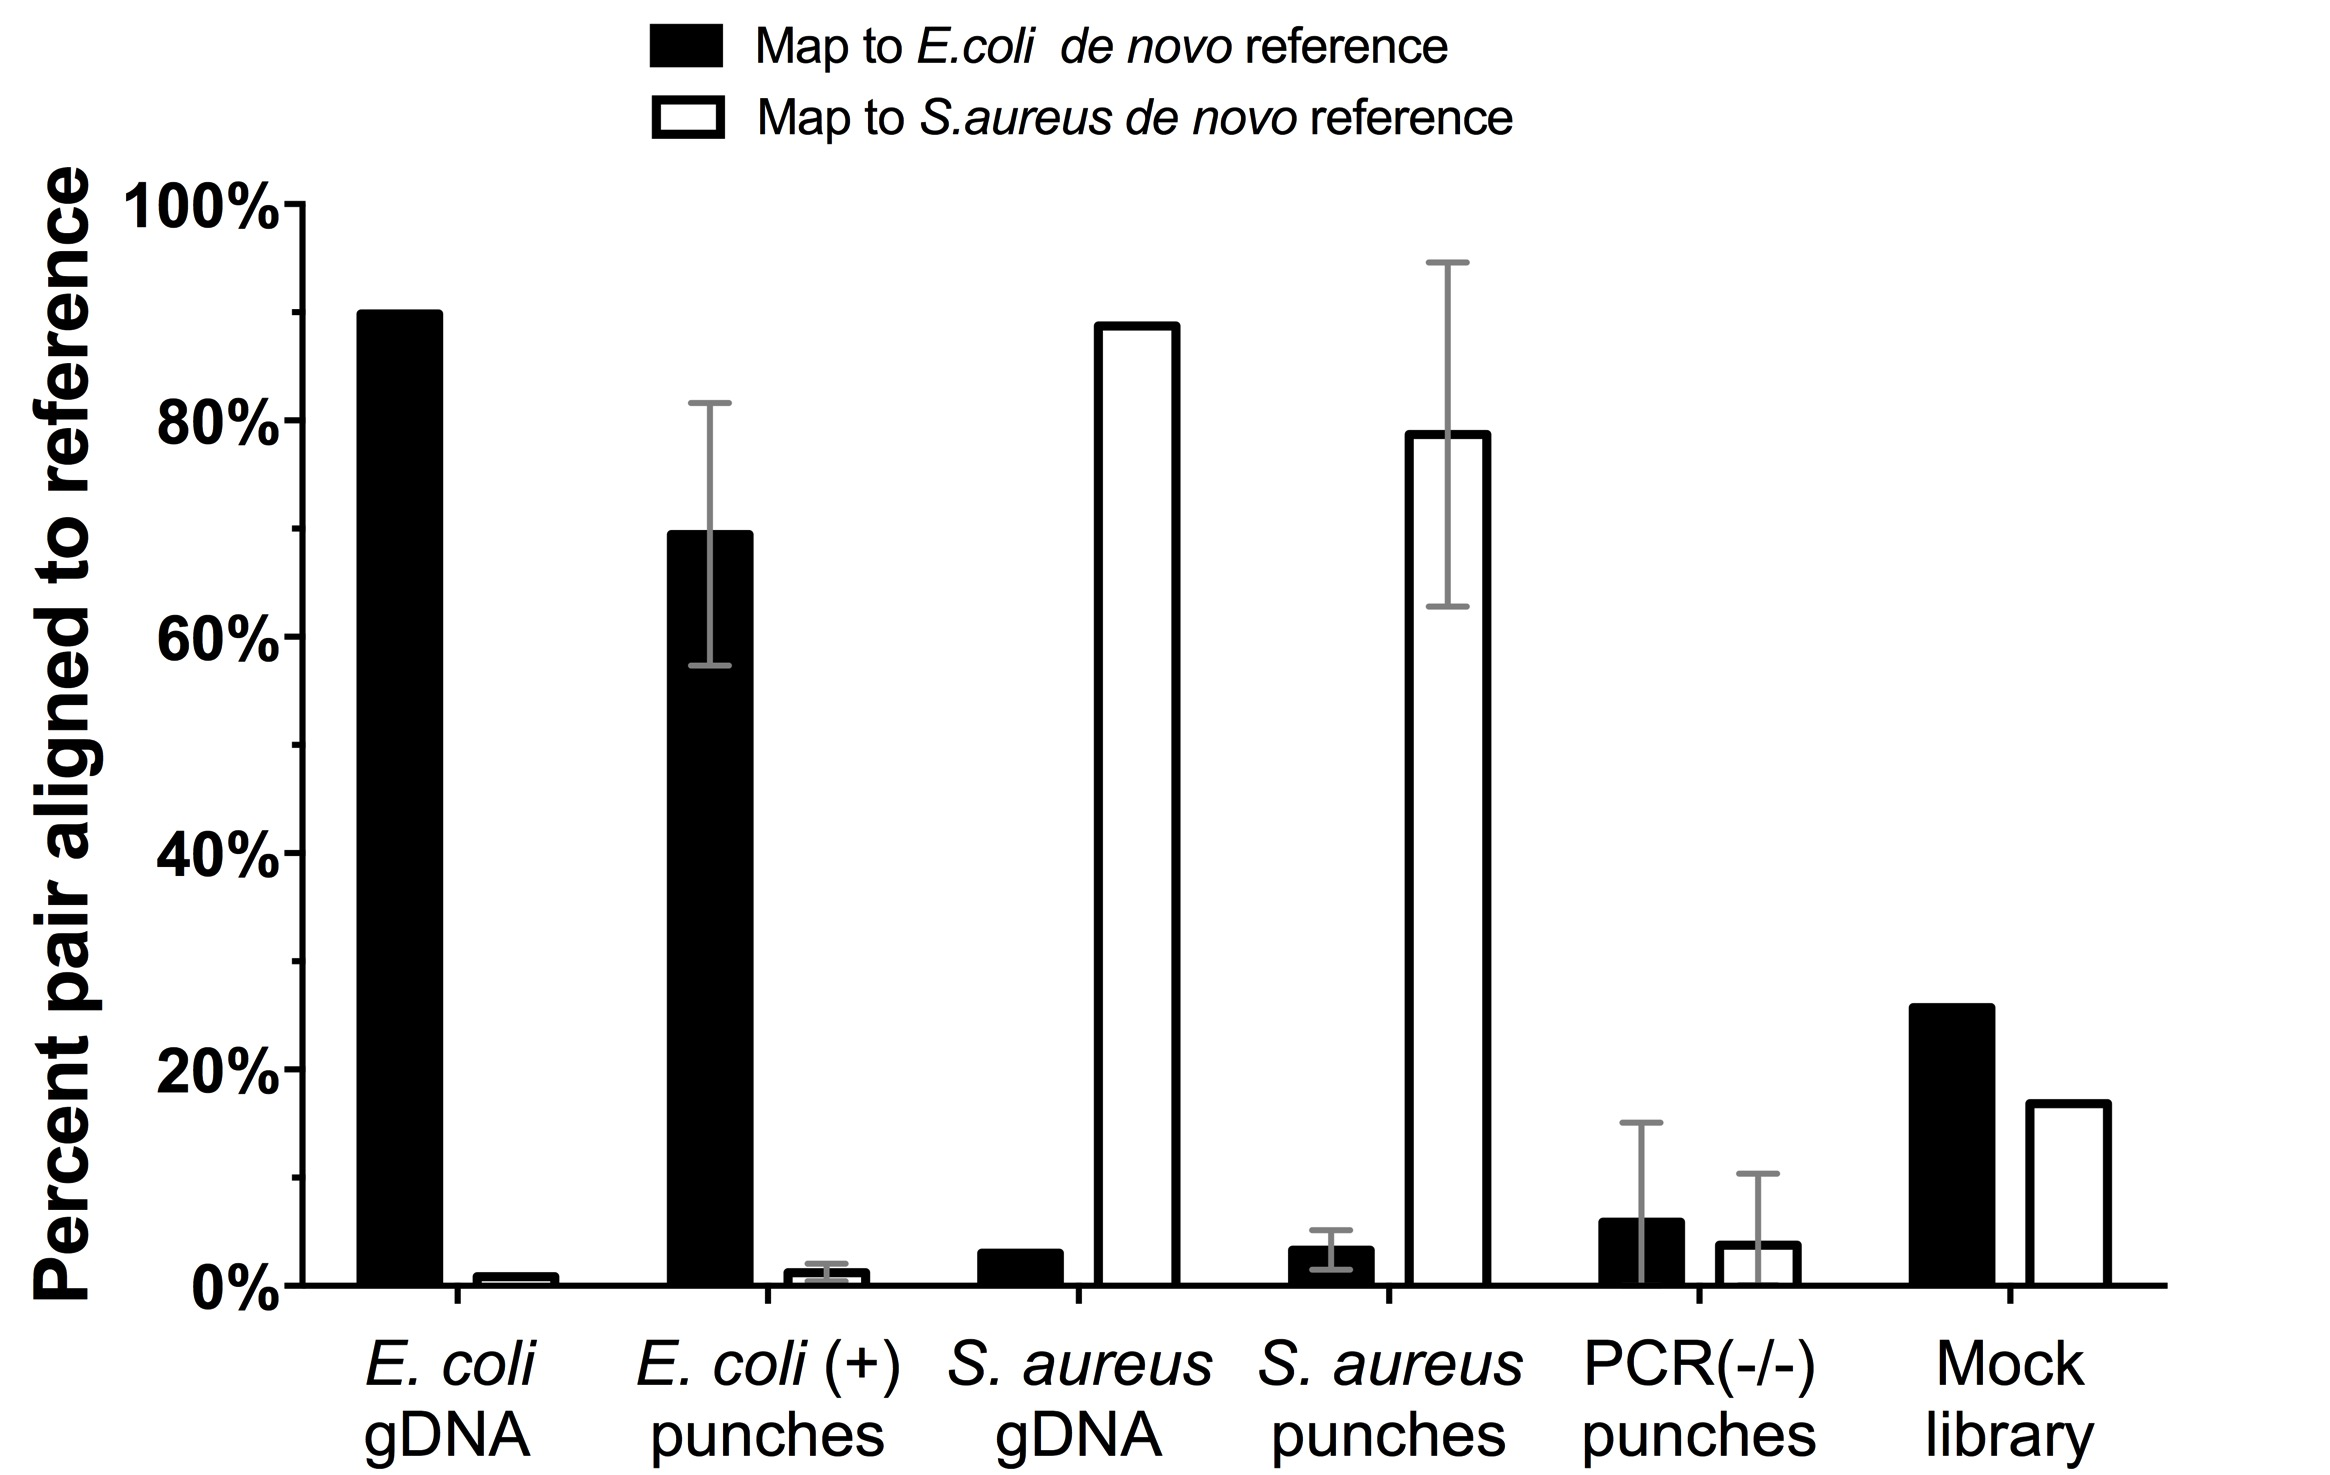
\includegraphics[keepaspectratio,width=0.6\textwidth]{./figures/SuppFig7.jpg}
\caption[Mapping single-cell genomes to references]{Mapping single-cell genomes to references. Single-cell samples were mapped to \textit{E. coli} and \textit{S. aureus} reference sequences with mean percent pair aligned and standard deviation shown. (n = 5 for \textit{E. coli} punches, n = 7 for \textit{S. aureus}, n = 7 for negative punches).}
\label{fig:MappingES}
\end{figure}

\begin{table}
\caption{Mapping statistics, \textit{E. coli} and \textit{S. aureus}}
\label{tab:MapStatES}

\includegraphics[width=\linewidth]{./figures/MapStatES}
\end{table}

Genome Coverage Completeness Estimation: note that some studies in the field report data from quality-filtered (`cherry-picked') cells, which dramatically improves quality statistics such as average coverage. In this study, we report data on complete sets of single-cell MDA reactions. 

\subsection{Custom reference generation by de novo assembly for \textit{E. coli} and \textit{S. aureus}}
The gDNA \textit{E. coli} (BL21) and \textit{S. aureus} (8325) positive-control data were assembled and curated to create custom reference genome sequences. Raw sequencing files were quality trimmed using Trimmomatic (Fig. \ref{fig:ESDataAnalysis}). We blasted the trimmed files against respective reference database and filtered described previously with the parameters listed in in Fig. \ref{fig:ESDataAnalysis}. Hit reads were filtered out of the sequencing files using QIIME filter\_fasta.py tool. The filtered and trimmed files were assembled into unordered contigs with velvet. We mapped (BWA) unordered contigs to their closest NCBI reference genome (NC\_012971 and NC\_007795.1 respectively). The resulting SAM files were ranked on mapped length in descending order. Using a custom MATLAB function, we created a reference genome backbone consisting of only `-' with the same size as the reference genome and wrote sequences on it with only the top SAM mapping sequence for each contig. We conducted the same assembly process for the genomic DNA (\textit{E. coli} DH10B) data from de Bourcy \textit{et al.} 2014 using reference genome NC\_010473.1. Assembly Statistics are listed in Table \ref{tab:deNovoAssemblyES}. Custom MATLAB function, python codes and shell scripts are included in the supplementary software zip file in Xu \textit{et al.} 2016. 

\begin{table}
\caption{\textit{de novo} assembly statistics, \textit{E. coli} and \textit{S. aureus}}
\label{tab:deNovoAssemblyES}
\begin{center}
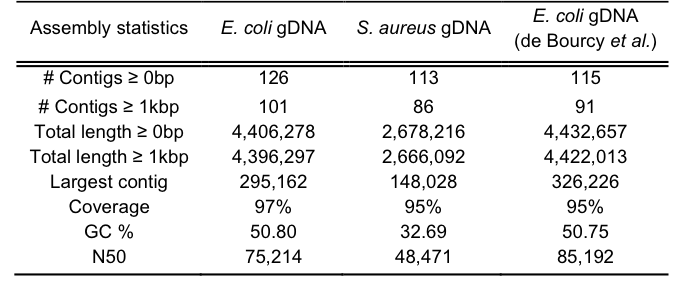
\includegraphics[width=0.85\linewidth]{./figures/deNovoAssemblyES}
\end{center}
\end{table}

Random subsampling of mapped reads for \textit{E. coli} and \textit{S. aureus}
Duplicates-marked BAM files were down-sampled using samtools and bootstrapped with random number seed 0 to 9 for each depth. See Table \ref{tab:DownsamplingESD} for more information. 

\begin{table}
\caption{Downsampling on mapped reads from single-cell MDA samples}
\label{tab:DownsamplingESD}

\includegraphics[width=\linewidth]{./figures/DownsamplingESdeBourcy}
\end{table}

% Need to rework 
\subsection{Chimera statistics for \textit{E. coli} and \textit{S. aureus}}
To make the chimera statistics comparable, we used \textit{de novo} assembled genome sequences (described below) from bulk genomic DNA samples as the reference. We mapped read 1 and read 2 from each sample single-ended using BWA. We sorted the SAM file by read index. We used a custom python code to import pysam in order to pair up the `read index', `mapping position', `is-reverse', and `read length' information into a .mat file. With a customized MATLAB script, we calculated the insert size for each read pair and checked their relative orientation. We filtered out pairs that were mapped one-ended. The chimera percentage was calculated as the (number of properly orientated read pairs with insert size more than 1000 bp + number of read pairs of wrong orientation)\slash Total number of read pairs.

\subsection{In-gel single-microbe MDA - human gut microbiome samples}
We received ethics approvals for human subjects research from the Columbia University IRB, Massachusetts Institute IRB, Broad Institute IRB, and two research ethics committees in Fiji: HRERC at CMNHS, FNU and FNHRERC at MoHFiji Ministry of Health. Fiji Community Microbiome Project (FijiCOMP) study participants from 5 agrarian villages within the Fiji Islands provided stool samples stored in 20\% glycerol within 30 minutes of voiding and were frozen at --80$^{\circ}$C (Five participants: M1.20, W2.21, WL.26, W2.33, M2.41) (Table \ref{tab:MetagenomicFiji}). 10 $\mu$L of thawed cells were resuspended in 500 $\mu$L PBST (0.1 \%). Samples were sonicated for 20 seconds and filtered through 35 $\mu$m Nylon mesh and 5 $\mu$m membrane (Pall Corp.) to collect filtrate with a 500 $\mu$L PBST wash. Samples were further diluted 1 to 500 $\sim$ 1 to 2000 fold in PBST to reach the final concentration of $\sim$ 30 cells\slash $\mu$L. The diluted cell samples (2 $\mu$l) then underwent alkaline lysis (1.5 $\mu$L D2 buffer) for 15 minutes at room temperature, after which the solution was neutralized (1.5 $\mu$L Stop solution). Hydrogel monomer mix (1.3 mg 4-Arm PEG Acrylate and 0.9 mg SH-PEG-SH) and MDA master mix were pipetted gently down the wall of each sample tube. MDA master mix includes 1$\times$ phi 29 buffer (NEB), 50 $\mu$M random hexamers with two phosphorothioate bonds at 3' terminus, 2.5 \% DMSO, 0.4 mM dNTP, 0.5 mg\slash mL BSA, 500 nM SYTOX Orange (Invitrogen) and 1 $\mu$L REPLI-g SC Polymerase (Qiagen). Only gentle tapping was used to ensure reagent mixing, in order not to disrupt the lysed microbes and denatured genomes. 25 $\mu$L of each microbial suspension was added into a frame-seal chamber, the sealed chamber was incubated at 30 $^{\circ}$C for 12 hours, followed by 65 $^{\circ}$C for 5 mins.

\begin{table}
\caption{Metagenomic shotgun profiling weighted with single-cell samples}
\label{tab:MetagenomicFiji}

\includegraphics[width=\linewidth]{./figures/MetagenomicShotgunProfilingFiji}
\end{table}

\paragraph{Secondary In-gel MDA - human gut microbiome samples}
Hydrogel punches (approximately 0.24 $\mu$L of hydrogel and 10 pg of DNA if a cluster was captured) were dissolved and denatured in 1 $\mu$L of 400 mM KOH with 0.1 mM EDTA and 0.1 M DTT at 72 $^{\circ}$C for 10 min before neutralization in 1 $\mu$L stop solution (Qiagen REPLI-g single cell kit). The neutralized product was added to 8 $\mu$L hydrogel and MDA master mix to reach a final volume of 10 $\mu$L for second round MDA reaction in hydrogel. The MDA reaction was incubated for 10 hours at 30 $^{\circ}$C before polymerase deactivation at 65 $^{\circ}$C for 5 min. The 10 $\mu$L gel was dissolved with 10 $\mu$L 400 mM KOH for 5mins at 72$^{\circ}$C, and then neutralized with 6.6 $\mu$L 2.5\% acetic acid.

\paragraph{Pre-processing and assembly of single-cell genomes from stool}
First, we removed the adapter sequences from single-cell libraries using TRIMMOMATIC \cite{Bolger:2014ek} (TRAILING:3 MINLEN:40). To ensure that human DNA was not captured in our single-cell libraries, we screened single-cell amplicons against the human genome (GRCh38 reference) using BMTagger \cite{Rotmistrovsky:CVigB6Il}(default). We screened our amplicons against \textit{E. coli} references (BL21 and DH10B) using BMTagger. Overall, the level of contamination was small. We also screened against \textit{Pseudomonas} (PAO1) and \textit{Staphylococcus} (NCTC 8325) genomes, which were sequenced alongside our libraries, to ensure no chimeric reads formed during sample preparation with contaminating sequences from other cultures in our lab that confounded our analyses. Finally, single genome amplicons were quality filtered (Phred score > 3), and filtered for reads that were less than 45 bp. Amplicons were then assembled using SPAdes (v3.6.0) (--careful) \cite{Bankevich:2012ih}. We retained genomes where at least 100 kb could be assembled.

\paragraph{Assessing the fidelity of single-cell genomes from stool}
To further vet the quality and purity of our assemblies, we used BLAST to assign taxonomies to a set of 31 predetermined core genes that are both phylogenetically conserved and single copy in almost all genomes \cite{Wu:2012dh}. Although we could not identify the full set of 31 core genes in any of the assemblies, we were able to easily distinguish cases where two or more cells were sequenced together from those in which there was a single cell. Additional validation of the single-cell assemblies included quantifying the levels of contamination using CheckM \cite{Parks:2015hs} and examining the number and taxonomy identified using RNAmmer \cite{Lagesen:2007ud}. CheckM accesses the quality of a genome using a broader set of marker genes specific to its inferred lineage within a reference genome tree and provides estimates of genome completeness and contamination percentages. RNAmmer uses hidden Markov models trained from ribosomal RNA databases to predict the rRNA species. The extent and contiguity of our assemblies was documented by reporting assembled genome size, N50, the number of contigs, CheckM completeness \%, CheckM contamination \% and notes on RNAmmer classification in an excel file in Xu \textit{et al.} 2016.

Notably, some microbes can be difficult to isolate from human stool samples due to the cells' tendency to break or aggregate. Some of the punch samples with low numbers of AMPHORA genes could be the result of broken cells containing reduced genomic representation or free genomic DNA fragments, while samples with evidence for multiple taxonomies could have resulted from cell aggregates. Stool samples are also fairly complex and contain a lot particulate matter that complicates sample processing. In principle, genes from samples with sequences of variable taxonomy could arise for several reasons: the products of multiple cells being collected in a single punch, downstream contamination in the second round MDA or library construction steps, informatic demultiplexing, or from taxonomic mis-classification of hard-to-assign sequences.

\paragraph{Analysis of metagenomic shotgun reads from stool}
FijiCOMP metagenomic samples, each containing roughly 50 million paired-reads, were profiled using MetaPhlAn \cite{Segata:2012ts}. Metagenomic samples were also aligned to the SILVA rRNA database (v.115) to determine the presence of organisms from the Succinivibrionaceae family. Based on alignments to the SILVA rRNA database, we find that organisms within the Succinivibrionaceae family are in fact highly abundant in the FijiCOMP metagenomic data, with average FPKM (Fragments Per Kilobase of transcript per Million mapped reads) values around 26,000.

\subsection{Accession codes}
Raw sequencing data on \textit{E. coli} and \textit{S. aureus} are accessible at the NCBI Sequence Read Archive (SRA) under BioProject accession number PRJNA279815 with BioSample accession numbers SAMN03451478-SAMN03451501. FijiCOMP metagenomic reads can be found under BioProject accession number PRJNA217052 with the accession numbers: SRX345831, SRX344363, SRX344765, SRX343094, SRX344442, SRX346405, SRX343839, SRX343780, SRX345901, SRX344600, SRX343866, SRX343411, SRX344189, SRX344380, SRX346966, SRX345329, SRX343800, and SRX344616. FijiCOMP virtual microfluidics 117 single cells are accessible with the BioSample accession numbers SAMN04461233-SAMN04461349.


% From Brito et al.
% ``However, despitethe high prevalence of genes and broader gene functions, we found that 34.9\% of the gene contexts, defined as the set of unique combinations between adjacent genes that were observed, were specific to individuals; very few of these gene contexts were conserved across populations''
% ``Together, high recombination rates and population-specificity support the notion that environmental selection on individual genes, rather than dispersal limitation alone, plays a key role in driving gene abundances.''
% ``Second, even though each of the mobile genes within our data set exists in more than one species, some of those genes may be primarily associated with a single taxon. This is especially true if a single taxon is much more abundant than the other species that carry the gene''
% ``We also showed that the mobile genetic elements are highly diverse among individuals, raising the possibility that they may vary within bacterial lineages in an individual over short time spans.''

% References:
% ``Some single-cell MDA products will not yield 16S rRNA gene PCR amplification products. Reasons for this can include the lack of these genomics regions in the amplified DNA due to the amplification bias (see below) or mismatches of the universal 16S rRNA primers, which will prevent amplification of 16S rRNA genes in certain taxa (e.g., Baker et al., 2003, 2010; Youssef et al., 2014).''